\chapter{StrepHit}
\label{cha:strephit}
La terza parte del progetto consiste nell'implementazione di uno script in Python (versione 2.7) che, dato in input un dataset di QuickStatements, deve restituire in output il dataset
arricchito con nuovi riferimenti.

Ogni riga del dataset di input presenta una proprietà \code{P854} (reference URL~\cite{P854}) con abbinata l'URL di riferimento della risorsa; 
lo script deve eseguire una query SPARQL per trovare l'item nel knowledge-base di Wikidata che corrisponde/identifica il dominio della URL. 
Se questo item di Wikidata esiste allora si cerca anche una e la proprietà di tale item che definisca uno schema\footnote{
    \textbf{Schema della URL}, in Wikidata esiste una proprietà \code{P1630} (formatter URL~\cite{P1630}) che definisce un template generale per una categoria di URL. 
    Per esempio una \textit{formatter URL} può essere la seguente: \code{http://www.nndb.com/people/$\$$1/} dove $\$1$ è un placeholder che rappresenta una qualsiasi stringa.  
} valido per l'URL in questione.

\section{Esempio di funzionamento}
Per esempio dato il seguente Quickstatement in input:
\begin{lstlisting}[style=QuickstatementsStyle, caption=Riga del dump]
    Q193660	P106	Q207628	S854	"http://www.nndb.com/people/031/000097737/"
\end{lstlisting}

Notiamo una prima relazione semantica 
\code{Q193660} (Ramon Llull~\cite{Q193660}) 
\code{P106} (occupation~\cite{P106}) 
\code{Q207628} (musical composition~\cite{Q207628}) 
che ci dice semplicemente che \qt{Ramon Llull lavora come compositore musicale}.

Segue la proprietà, di maggiore interesse, \code{S854 "http://www.nndb.com/people/031/000097737/"} che indica la provenienza dell'informazione. 

Lo script procede estrapolando il dominio dalla reference url (\code{www.nndb.com}) e, con una query SPARQL, cerca un item di riferimento per tale dominio in Wikidata 
(non è sempre garantita la presenza).

In questo esempio l'item di riferimento è \code{Q1373513} (NNDB~\cite{Q1373513}) perchè presenta la proprietà \code{P856} (official website~\cite{P856}) che corrisponde al dominio cercato;
lo stesso item ha anche una proprietà chiamata \qt{Wikidata property} (\code{P1687}) con abbinato l'identificativo di un'altra proprietà chiamata  
\qt{NNDB people ID} (\code{P1263}).

Se andiamo ad analizzare la proprietà \qt{NNDB people ID} (\code{P1263}~\cite{P1263}) notiamo che presenta a sua volta una proprietà 
\qt{formatter URL} (\code{P1630}~\cite{P1630}) il cui valore è \code{http://www.nndb.com/people/$\$1/$}. 
Il valore finale \code{$\$1$} nella \textit{formatter URL}\rq\rq\ è un placeholder che sta ad indicare la parte della URL che corrisponde al valore della proprietà prescelta. 

In questo esempio avremmo:
\begin{lstlisting}[style=QuickstatementsStyle, caption=Esempio di formatter URL]
    URL originale presente nel dump:        http://www.nndb.com/people/031/000097737/
    Formatter URL:                          http://www.nndb.com/people/$1/
    Valore della proprieta':                031/000097737
    (estrapolato grazie al placeholder $1)
\end{lstlisting}

Lo script andrà quindi ad estrapolare dalla URL di partenza la stringa \code{031/000097737} che corrisponde al valore della proprietà \code{P1263} e andrà ad arricchire il dump 
con questa informazione aggiuntiva.

\begin{lstlisting}[style=QuickstatementsStyle, caption=Risultato dello script]
    Q193660	P106	Q207628	S854	"http://www.nndb.com/people/031/000097737/"	S248	Q1373513	S1263	"031/000097737"	S813	2018-06-04T02:19:10Z/14
\end{lstlisting}

I riferimenti aggiuntivi sono: 
\code{S248} (stated in~\cite{P248})
\code{Q1373513} (NNDB~\cite{Q1373513})
\code{S1263} (NNDB people ID~\cite{P1263})
\code{"031/000097737"} (il valore estrapolato, people ID)
\code{S813} (retrieved~\cite{P813})
\code{2018-06-04T02:19:10Z/14} (timestamp).

\section{SPARQL Query}
Per risolvere ogni dominio e ogni \qt{formatter URL} sconosciuta si usa una sola query; si è cercato di limitare il più possibile il numero di query effettuate 
(dato che alcune query possono impiegare svariati secondi per essere eseguite), 
salvando in memoria e su disco i risultati di quelle già lanciate in precedenza per minimizzare il tempo di computazione dello script.

\begin{lstlisting}[style=SPARQLStyle, caption=SPARQL query per cercare item e proprietà relativi al dominio \code{"www.nndb.com"}]
    select Distinct ?subjects ?wikidataProperty ?formatterUrlLabel ?sitelinkLabel
    where {
        {
            BIND("www.nndb.com" AS ?domain).
            SERVICE wikibase:label { bd:serviceParam wikibase:language "[AUTO_LANGUAGE],en". }
            ?subjects wdt:P856 ?sitelink ;
                      wdt:P1687 ?wikidataProperty.
            ?wikidataProperty wdt:P1630 ?formatterUrl
            FILTER (REGEX(str(?formatterUrl), ?domain) || REGEX(str(?sitelink), ?domain)).
        }
        union
        {
            BIND("www.nndb.com" AS ?domain).
            SERVICE wikibase:label { bd:serviceParam wikibase:language "[AUTO_LANGUAGE],en". }
            ?subjects wdt:P856 ?sitelink ;
            FILTER REGEX(str(?sitelink), ?domain).
        }
    }
\end{lstlisting}

Va premesso che esistono molti modi per ottenere lo stesso risultato, con costrutti molto meno verbosi, tuttavia questa è l'unica query trovata che attualmente non manda in timeout l'endpoint.

Il superamento del timeout è sicuramente dovuto al fatto che internamente si usano delle regular expressions che appesantiscono molto l'esecuzione della query, soprattutto su 
grandi knowledge-base come quello di Wikidata. 

In SPARQL usare una ricerca per stringa è certamente una forzatura perchè solitamente si conoscono già a priori item e propery che interessano tuttavia, in questo caso, è 
stato necessario adottare la ricerca per regular expression dato che lo script deve proprio affrontare il problema inverso.

La query è il risultato dell'unione di due sub-query; la prima sub-query cerca tutte le proprietà che posseggono una proprietà \qt{formatter URL} (\code{P1630}) il cui valore ha come dominio quello del 
Quickstatement che lo script sta analizzando (in questo caso \code{"www.nndb.com"}); in oltre controlla che tale priprietà sia legata ad un item il cui \qt{official website} (\code{P856}) 
sia coerente con il dominio in questione. 

La seconda sub-query invece cerca tutti gli item il cui \qt{official website} (\code{P856}) abbia lo stesso dominio di quello del Quickstatement che lo script sta analizzando. 
Questa query è necessaria perchè non sempre esiste una proprietà la cui \qt{formatter URL} sia coerente con il link che si sta analizzando; può succedere che esista solo l'item 
relativo al database in questione ma non la proprietà specifica, in pochi casi non esiste nemmeno tale item. 

In alcuni casi può succedere che l'item relativo al database esista ma abbia un dominio completamente differente da quello della proprietà la cui \qt{formatter URL}
presenta un match con l'URL in analisi. 

La difficoltà principale nella realizzazione dello script è stata proprio quella di gestire una moltitudine di casi particolari, derivanti dal fatto che il dataset è molto grande
(più di 500.000 Quickstatements) ed eterogeneo (presenta svariati domini differenti e qualche URL completamente sbagliata o deprecata). 

\begin{center}
    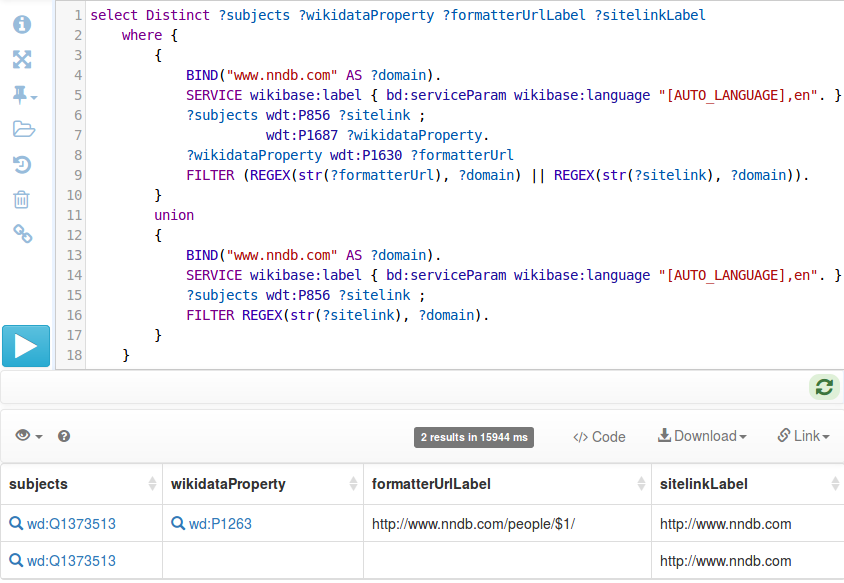
\includegraphics[width=\linewidth]{Sources/Img/c04_01.png}
    \captionof{figure}{Risultato della query per il dominio \code{"www.nndb.com"}}
\end{center}

\section{Lo script}

\subsection{Struttura del progetto}
Il progetto presenta una cartella \qt{assets} contenente tutti i file di input e output, i \code{.json} di configurazione e i \code{.log} degli errori; 
nella cartella \qt{business} sono contenuti i servizi, i metodi di utilità e le query. 

La cartella \qt{domain} contiene i modelli e le localizations (nel file \code{localizations.py} sono definite anche una serie di costanti da settare a seconda 
delle esigenze per configurare lo script). 

In \qt{tests} abbiamo tutte le classi di test basate sulla libreria unittest~\cite{unittest}; come per il Client $C\#$ anche in questo caso è stato configurato Travis per far eseguire i test 
automaticamente ad ogni pull-request. 

Infine nella root del progetto abbiamo l'entry point dello script (\code{main.py}) e l'entry point dei test (\code{test.py}), i requirement per il package manager 
e il file di configurazione \code{strephit.py}, nel caso si voglia lanciare lo script in un virtualenv~\cite{virtualenv} tramite la libreria Click~\cite{click}.

\subsection{Algoritmo}
Istanziando l'oggetto \code{QuickStatementsService} vengono caricati automaticamente in memoria i \code{mappings} presenti nella cartella \qt{assets}; 
i \code{mappings} sono dei file \code{.json} in cui lo script salva i risultati delle le chiamate, all'endpoint SPARQL, già effettuate.

\begin{lstlisting}[style=jsonStyle, caption=Some Code]
    "www.nndb.com": [
        {
            "db_id": "Q1373513", 
            "db_property": "S1263", 
            "to_upper_case": false, 
            "url_pattern": "http://www.nndb.com/people/$1/"
        }
    ], 
\end{lstlisting}

Il metodo \code{add\u db\u references\u async()} cicla su ogni riga del dataset e per ogniuna di esse chiama un handler 
(\code{add\u db\u references\u async\u handler()}), passandogli un oggetto \code{QuickStatement} contenente tutte le informazioni della riga, 
che procede con l'analisi dell'URL e la generazione dei riferimenti mancanti.

A questo punto, in modo sincrono o asincrono, a seconda del settaggio delle costanti in \code{localizations.py} (\code{IS\u ASYNC \u MODE = True/False}), 
viene chiamato il metodo \code{generate\u db\u reference()} che provvede a controllare che nei \code{mappings} ci sia già una entry con formatter URL compatibile 
con l'URL del Quickstatement e a generare i riferimenti mancanti.

Se nei \code{mappings} non esiste nessuna entry compatibile con l'URL viene chiamato il metodo \code{new\u mapping()} che provvede a chiamare l'endpoint SPARQL 
e a selezionare il risultato migliore per aggiungerlo ai \code{mappings}. 

Se la costante \code{MAP\u ALL\u RESPONSES} viene settata a \code{True}, ogni risposta del endpoint SPARQL viene salvata interamente nei \code{mappings};
questo previene qualsiasi altra chiamata all'endpoint per un determinato dominio ma accresce la dimensione dei \code{mappings} a dismisura, rendendo la ricerca più lenta.
 
\subsection{Refresh delle URL}
Nel dataset analizzato alcuni domini sono deprecati tant'è che tentando di accederci con un browser si viene reindirizzati ad altri domini oppure si passa da http ad https.

Per non perdere questi riferimenti si è deciso di implementare anche una funzionalità che data una lista di domini va a fare un \qt{refresh} di tutte le URL aventi tali domini 
e ad eliminare le righe contenenti URL inesistenti.

A fine procedura vengono salvati i \code{.log} con la lista delle URL modificate e delle righe eliminate dal dataset.

